% Options for packages loaded elsewhere
\PassOptionsToPackage{unicode}{hyperref}
\PassOptionsToPackage{hyphens}{url}
%
\documentclass[
  ignorenonframetext,
]{beamer}
\usepackage{pgfpages}
\setbeamertemplate{caption}[numbered]
\setbeamertemplate{caption label separator}{: }
\setbeamercolor{caption name}{fg=normal text.fg}
\beamertemplatenavigationsymbolsempty
% Prevent slide breaks in the middle of a paragraph
\widowpenalties 1 10000
\raggedbottom
\setbeamertemplate{part page}{
  \centering
  \begin{beamercolorbox}[sep=16pt,center]{part title}
    \usebeamerfont{part title}\insertpart\par
  \end{beamercolorbox}
}
\setbeamertemplate{section page}{
  \centering
  \begin{beamercolorbox}[sep=12pt,center]{part title}
    \usebeamerfont{section title}\insertsection\par
  \end{beamercolorbox}
}
\setbeamertemplate{subsection page}{
  \centering
  \begin{beamercolorbox}[sep=8pt,center]{part title}
    \usebeamerfont{subsection title}\insertsubsection\par
  \end{beamercolorbox}
}
\AtBeginPart{
  \frame{\partpage}
}
\AtBeginSection{
  \ifbibliography
  \else
    \frame{\sectionpage}
  \fi
}
\AtBeginSubsection{
  \frame{\subsectionpage}
}
\usepackage{lmodern}
\usepackage{amsmath}
\usepackage{ifxetex,ifluatex}
\ifnum 0\ifxetex 1\fi\ifluatex 1\fi=0 % if pdftex
  \usepackage[T1]{fontenc}
  \usepackage[utf8]{inputenc}
  \usepackage{textcomp} % provide euro and other symbols
  \usepackage{amssymb}
\else % if luatex or xetex
  \usepackage{unicode-math}
  \defaultfontfeatures{Scale=MatchLowercase}
  \defaultfontfeatures[\rmfamily]{Ligatures=TeX,Scale=1}
\fi
% Use upquote if available, for straight quotes in verbatim environments
\IfFileExists{upquote.sty}{\usepackage{upquote}}{}
\IfFileExists{microtype.sty}{% use microtype if available
  \usepackage[]{microtype}
  \UseMicrotypeSet[protrusion]{basicmath} % disable protrusion for tt fonts
}{}
\makeatletter
\@ifundefined{KOMAClassName}{% if non-KOMA class
  \IfFileExists{parskip.sty}{%
    \usepackage{parskip}
  }{% else
    \setlength{\parindent}{0pt}
    \setlength{\parskip}{6pt plus 2pt minus 1pt}}
}{% if KOMA class
  \KOMAoptions{parskip=half}}
\makeatother
\usepackage{xcolor}
\IfFileExists{xurl.sty}{\usepackage{xurl}}{} % add URL line breaks if available
\IfFileExists{bookmark.sty}{\usepackage{bookmark}}{\usepackage{hyperref}}
\hypersetup{
  pdftitle={Clase 10 Inferencia estadística},
  pdfauthor={Dr.~José A. Gallardo \textbar{} jose.gallardo@pucv.cl \textbar{} Pontificia Universidad Católica de Valparaíso},
  hidelinks,
  pdfcreator={LaTeX via pandoc}}
\urlstyle{same} % disable monospaced font for URLs
\newif\ifbibliography
\usepackage{longtable,booktabs}
\usepackage{calc} % for calculating minipage widths
\usepackage{caption}
% Make caption package work with longtable
\makeatletter
\def\fnum@table{\tablename~\thetable}
\makeatother
\setlength{\emergencystretch}{3em} % prevent overfull lines
\providecommand{\tightlist}{%
  \setlength{\itemsep}{0pt}\setlength{\parskip}{0pt}}
\setcounter{secnumdepth}{-\maxdimen} % remove section numbering
\ifluatex
  \usepackage{selnolig}  % disable illegal ligatures
\fi

\title{Clase 10 Inferencia estadística}
\subtitle{Curso Introducción al Análisis de datos con R para la
acuicultura.}
\author{Dr.~José A. Gallardo \textbar{}
\href{mailto:jose.gallardo@pucv.cl}{\nolinkurl{jose.gallardo@pucv.cl}}
\textbar{} Pontificia Universidad Católica de Valparaíso}
\date{10 July 2021}

\begin{document}
\frame{\titlepage}

\begin{frame}{PLAN DE LA CLASE}
\protect\hypertarget{plan-de-la-clase}{}
\textbf{1.- Introducción}

\begin{itemize}
\tightlist
\item
  ¿Qué es la inferencia estadística?.\\
\item
  Conceptos importantes.
\item
  ¿Cómo someter a prueba una hipótesis?
\item
  Interpretar resultados de análisis de datos con R.
\end{itemize}

\textbf{2.- Práctica con R y Rstudio cloud}

\begin{itemize}
\tightlist
\item
  Realizar pruebas de hipótesis: Correlación, comparación de medias (2
  muestras independientes y pareadas).
\item
  Realizar gráficas avanzadas con ggplot2.
\item
  Elaborar un reporte dinámico en formato pdf.
\end{itemize}
\end{frame}

\begin{frame}{INFERENCIA ESTADÍSTICA}
\protect\hypertarget{inferencia-estaduxedstica}{}
\textbf{¿Qué es la inferencia estadística?}

Son procedimientos que permiten obtener o extraer conclusiones sobre los
parámetros de una población a partir de una muestra de datos tomada en
ella.

\textbf{¿Qué inferencia puede hacer de este experimento?}

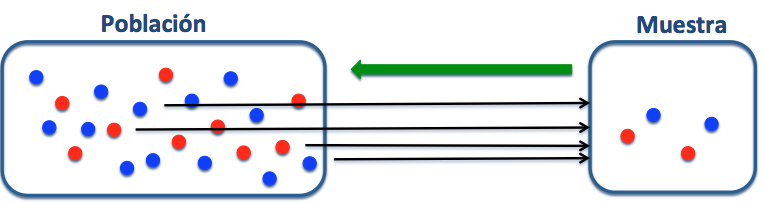
\includegraphics[width=1\linewidth]{Inferencia}
\end{frame}

\begin{frame}{INFERENCIA ESTADÍSTICA 2}
\protect\hypertarget{inferencia-estaduxedstica-2}{}
\textbf{¿Para qué es útil?}

\begin{itemize}
\item
  \textbf{Es más económico que hacer un Censo.}\\
  ¿Cuál es la biomasa en un estanque?\\
  ¿Cuántas larvas tengo para sembrar?
\item
  \textbf{Bajo ciertos supuestos permite hacer afirmaciones.}\\
  Si alimento mis camarones con la dieta A crecerán más que con la dieta
  B.\\
  La eficacia de la vacuna es menor cuando los peces sufren una
  coinfección de patógenos.
\end{itemize}
\end{frame}

\begin{frame}{CONCEPTOS IMPORTANTES}
\protect\hypertarget{conceptos-importantes}{}
\begin{itemize}
\tightlist
\item
  \textbf{Parámetro} Constante que caracteriza a todos los elementos de
  un conjunto de datos de una población. Se representan con letras
  griegas.
\end{itemize}

Promedio de una población (mu) = \(\mu\).

\begin{itemize}
\tightlist
\item
  \textbf{Estadístico} Una función de una muestra aleatoria o
  subconjunto de datos de una población.
\end{itemize}

Promedio de una muestra (\(\bar{X}\)) = \(\sum\) \(\frac{X_i}{N}\)
\end{frame}

\begin{frame}{ESTIMACIÓN DE UN PARÁMETRO}
\protect\hypertarget{estimaciuxf3n-de-un-paruxe1metro}{}
\textbf{Objetivo} Estimar parámetros de la población a partir de la
muestra de una variable aleatoria.

\textbf{Ejemplo} Estimar el promedio del peso del cuerpo de una
población a partir de una muestra de 30 animales.

\textbf{Tipos de estimación}

\begin{itemize}
\item
  \textbf{Estimación puntual}: Consiste en asumir que el parámetro tiene
  el mismo valor que el estadístico en la muestra.
\item
  \textbf{Estimación por intervalos}: Se asigna al parámetro un conjunto
  de posibles valores que están comprendidos en un intervalo asociado a
  una cierta probabilidad de ocurrencia.
\end{itemize}
\end{frame}

\begin{frame}{¿PUEDO ESTIMAR ERRONEAMENTE UN PARÁMETRO?}
\protect\hypertarget{puedo-estimar-erroneamente-un-paruxe1metro}{}
Por supuesto, muchos errores se producen por violar algunas premisas.

\begin{itemize}
\item
  \textbf{Las muestras deben tomarse de forma aleatoria.}\\
  No descartar animales pequeños en un muestreo (sobreestimo biomasa).
\item
  \textbf{Ley de los grandes números.}\\
  Mis variables están correlacionadas (3 muestras v/s 300 muestras).\\
  La biomasa del estanque es 100 kg (10 peces v/s 100 peces).
\item
  \textbf{Evitar sesgo del investigador}\\
  Deseo rechazar la hipótesis, repito hasta que rechazo.
\item
  \textbf{Otros}\\
  Errores y fraude.
\end{itemize}
\end{frame}

\begin{frame}{DISTRIBUCIÓN DEL ESTIMADOR}
\protect\hypertarget{distribuciuxf3n-del-estimador}{}
\begin{itemize}
\item
  \textbf{Distribución muestral del estimador}\\
  Dado que un estimador puntual (\(\bar{X}\)) también es una variable
  aleatoria, entonces también tiene una distribución de probabilidad.
\item
  \textbf{¿Cómo distribuye?}\\
  Si X \textasciitilde{} \emph{Normal}(\(\mu_{x}\),\(\sigma_{x}\))
\end{itemize}

Entonces el estimador de la media tiene \(\bar{X}\) \textasciitilde{}
\emph{Normal}(\(\mu_{x}\), \(\frac{\sigma_x}{\sqrt{N}}\))

\begin{itemize}
\tightlist
\item
  \textbf{¿Por qué es importante?}\\
  Conocer la distribución de \(\bar{X}\) nos permitirá hacer pruebas de
  hipótesis.
\end{itemize}
\end{frame}

\begin{frame}{PRUEBAS DE HIPÓTESIS}
\protect\hypertarget{pruebas-de-hipuxf3tesis}{}
\textbf{Objetivo} Realizar una afirmación acerca del valor de un
parámetro, usualmente contrastando con alguna hipótesis.

\textbf{Hipótesis estadísticas}\\
\emph{Hipótesis nula} (H\textsubscript{0}) es una afirmación, usualmente
de igualdad.

\emph{Hipótesis alternativa} (H\textsubscript{A}) es una afirmación que
se deduce de la observación previa o de los antecedentes de literatura y
que el investigador cree que es verdadera.

\textbf{Ejemplo}\\
\textbf{H\textsubscript{0}}: El peso medio de mis peces es igual a 1
Kg.\\
\textbf{H\textsubscript{A}}: El peso medio de mis peces es mayor a 1 Kg.
\end{frame}

\begin{frame}{¿POR QUÉ DOS HIPÓTESIS?}
\protect\hypertarget{por-quuxe9-dos-hipuxf3tesis}{}
\begin{itemize}
\item
  Las pruebas estadísticas tienen como propósito someter a prueba una
  hipótesis nula con la intensión de \emph{rechazarla}.
\item
  ¿Por qué no simplemente aceptar la alternativa?
\end{itemize}

\begin{quote}
We cannot conclusively affirm a hypothesis, but we can conclusively
negate it \emph{Karl Popper}
\end{quote}

\begin{itemize}
\item
  Pueden existir otros fenómenos no conocidos o no considerados que
  posteriormente permitan a otro investigador rechazar nuestra hipótesis
  alternativa.
\item
  Por lo tanto, los datos nos dirán si \textbf{existen o no } evidencias
  para rechazar la hipótesis nula.
\end{itemize}
\end{frame}

\begin{frame}{ETAPAS DE UNA PRUEBA DE HIPÓTESIS}
\protect\hypertarget{etapas-de-una-prueba-de-hipuxf3tesis}{}
Para cualquier prueba de hipotesis necesitas lo siguiente:

\begin{itemize}
\item
  Tus \emph{datos} (1).
\item
  Una \emph{hipótesis nula} (2).
\item
  La \emph{prueba estadística} (3) que se aplicará.
\item
  El \emph{nivel de significancuia} (4) para rechazar la hipótesis.
\item
  La \emph{distribución} (5) de la \emph{prueba estadística} respecto de
  la cual evaluarás la \emph{hipótesis nula} con el estadístico que
  estimas de tus \emph{datos}.
\end{itemize}
\end{frame}

\begin{frame}{PRUEBA DE HIPÓTESIS: NO RECHAZO.}
\protect\hypertarget{prueba-de-hipuxf3tesis-no-rechazo.}{}
\textbf{H\textsubscript{0}}: El peso medio de sus peces es igual a 1 Kg.

Si \textbf{\(\bar{X}\)} = 1,1 Kg, rechaza la hipótesis?

\includegraphics[width=0.7\linewidth]{Clase_07_Inferencia_estadistica_files/figure-beamer/unnamed-chunk-2-1}
\end{frame}

\begin{frame}{PRUEBA DE HIPÓTESIS: RECHAZO.}
\protect\hypertarget{prueba-de-hipuxf3tesis-rechazo.}{}
\textbf{H\textsubscript{0}}: El peso medio de sus peces es igual a 1 Kg.

Si \textbf{\(\bar{X}\)} = 1,2 Kg, rechaza la hipótesis?

\includegraphics[width=0.7\linewidth]{Clase_07_Inferencia_estadistica_files/figure-beamer/unnamed-chunk-3-1}
\end{frame}

\begin{frame}{¿CUÁNDO RECHAZAR \textbf{H\textsubscript{0}}?}
\protect\hypertarget{cuuxe1ndo-rechazar-h0}{}
\textbf{Regla de deisión}\\
Rechazo \textbf{H\textsubscript{0}} cuando la evidencia observada es
poco probable que ocurra bajo el supuesto de que la hipótesis sea
verdadera.

Generalmente \(\alpha\) = 0,05 o 0,01.

Es decir, rechazamos cuando el valor del estadístico está en el 5\%
inferior de la función de distribución muestral.

\textbf{Corrección de Bonferroni comparaciones múltiples}

Pero a veces \(\alpha\) = \(10^{-8}\)

Ejemplo: 50.000 genotipos asociados a un fenotipo. Solo por azar 2.500
estarán asociados con P \textless{} 0,05
\end{frame}

\begin{frame}{PRUEBA DE HIPÓTESIS: UNA COLA O DOS COLAS}
\protect\hypertarget{prueba-de-hipuxf3tesis-una-cola-o-dos-colas}{}
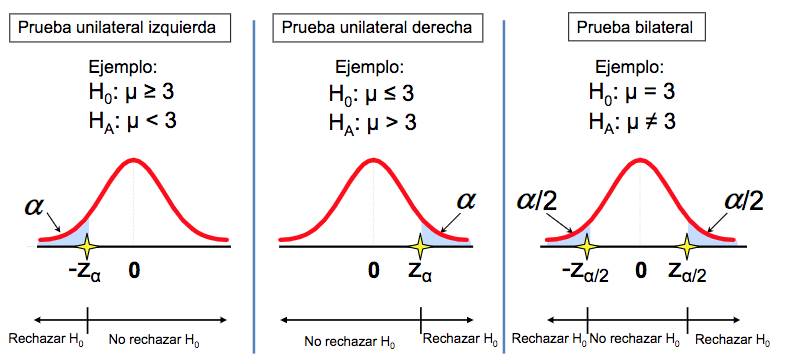
\includegraphics[width=1\linewidth]{region_rechazo}
\end{frame}

\begin{frame}{¿PUEDO COMETER UN ERROR EN LAS PRUEBAS DE HIPÓTESIS?}
\protect\hypertarget{puedo-cometer-un-error-en-las-pruebas-de-hipuxf3tesis}{}
Por supuesto, siempre es posible llegar a una conclusión incorrecta.

\textbf{Tipos de errores}\\
Tipo I (\(\alpha\)) y tipo II (\(\beta\)), ambos están inversamente
relacionados.

\begin{longtable}[]{@{}lll@{}}
\toprule
\textbf{Decisión} & \textbf{H\textsubscript{0} es cierta} &
\textbf{H\textsubscript{0} es falsa}\tabularnewline
\midrule
\endhead
\emph{Aceptamos H\textsubscript{0}} & Decisión correcta & Error tipo
II\tabularnewline
\emph{Rechazamos H\textsubscript{0}} & Error tipo I & Decisión
correcta\tabularnewline
\bottomrule
\end{longtable}
\end{frame}

\begin{frame}{SIGNIFICANCIA ESTADÍSTICA v/s PRÁCTICA}
\protect\hypertarget{significancia-estaduxedstica-vs-pruxe1ctica}{}
\begin{itemize}
\tightlist
\item
  \textbf{Problema 1}\\
  La vacuna aumenta significativamente el número de anticuerpos.
\end{itemize}

Sin vacuna = 10 anticuerpos Con vacuna = 11 anticuerpos (10 \% de
mejora).

¿Cuál es la importancia práctica de este hallazgo?

¿Mejorará la salud de mis peces?
\end{frame}

\begin{frame}{SIGNIFICANCIA ESTADÍSTICA v/s PRÁCTICA 2}
\protect\hypertarget{significancia-estaduxedstica-vs-pruxe1ctica-2}{}
\textbf{Problema 2} Si aumento N siempre lograré rechazar la hipótesis
nula, cada vez para diferencias más pequeñas. ¿Esto tiene significancia
práctica?

X e Y están significativamente correlacionados r = 0,01 (p-value =
0.01901)

\includegraphics[width=0.8\linewidth]{Clase_07_Inferencia_estadistica_files/figure-beamer/unnamed-chunk-6-1}
\end{frame}

\begin{frame}{SIGNIFICANCIA ESTADÍSTICA v/s PRÁCTICA 3}
\protect\hypertarget{significancia-estaduxedstica-vs-pruxe1ctica-3}{}
\textbf{Problema 3}

Clasificación basada en un punto de corte arbitrario.

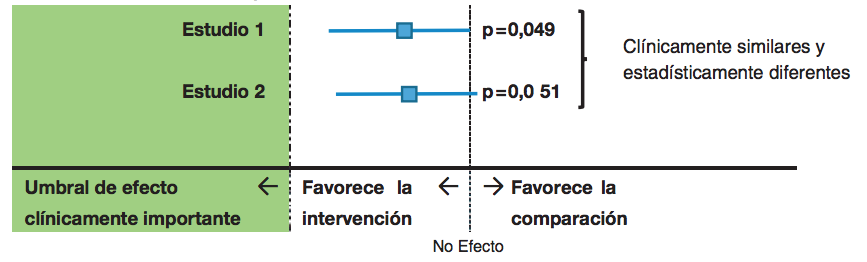
\includegraphics[width=1\linewidth]{punto_de_corte}
\end{frame}

\begin{frame}{SIGNIFICANCIA ESTADÍSTICA v/s PRÁCTICA 4}
\protect\hypertarget{significancia-estaduxedstica-vs-pruxe1ctica-4}{}
\textbf{Problema 4}\\
Resultados ``estadísticamente no significativos'' pueden ser o no ser
concluyentes.

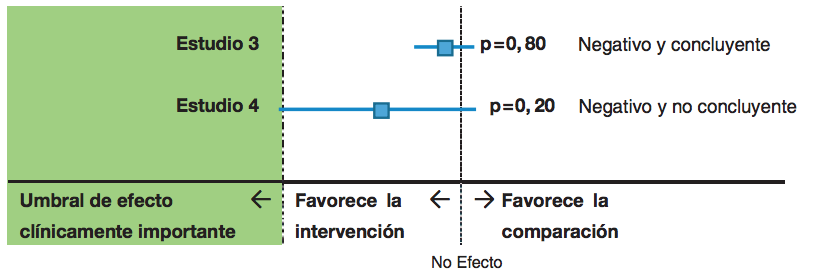
\includegraphics[width=1\linewidth]{no_concluyente}
\end{frame}

\begin{frame}{TÍPOS DE PRUEBAS ESTADÍSTICAS}
\protect\hypertarget{tuxedpos-de-pruebas-estaduxedsticas}{}
Según la forma de la distribución de la variable aleatoria.

\begin{itemize}
\tightlist
\item
  \textbf{Métodos paramétricos} Las pruebas de hipótesis usualmente
  asumen una distribución normal de la variable aleatoria.
\end{itemize}

Util para la mayoría de las variables cuantitativas continuas.

\begin{itemize}
\tightlist
\item
  \textbf{Métodos NO paramétricos} Las pruebas de hipótesis no asumen
  una distribución normal de la variable aleatoria.
\end{itemize}

Util para todas las variables, incluyendo cuantitativas discretas y
cualitativas.
\end{frame}

\begin{frame}{COEFICIENTE CORRELACIÓN DE PEARSON}
\protect\hypertarget{coeficiente-correlaciuxf3n-de-pearson}{}
\includegraphics[width=0.7\linewidth]{Clase_07_Inferencia_estadistica_files/figure-beamer/unnamed-chunk-9-1}

\textbf{Hipótesis} H0 : r = 0 ausencia de correlación H1 : r \(\neq\) 0
existencia de correlación

\textbf{Supuestos:} 1) Las variables X e Y son continuas y su relación
en lineal. 2) La distribución conjunta de (X, Y) es una distribución
Bivariable normal.
\end{frame}

\begin{frame}[fragile]{R Documentation cor.test \{stats\}}
\protect\hypertarget{r-documentation-cor.test-stats}{}
\begin{verbatim}
cor.test((x, y,
     alternative = c("two.sided", "less", "greater"),
     method = c("pearson", "kendall", "spearman"),
     conf.level* = 0.95, ...)
\end{verbatim}

\textbf{Pearson's product-moment correlation}

data: X - Y\\
t = 19.006, df = 1076, p-value \textless{} 2.2e-16\\
alternative hypothesis: true correlation is not equal to 0\\
95 percent confidence interval:\\
0.4552586 0.5447396\\
sample estimates:\\
cor: 0.5013383
\end{frame}

\begin{frame}{PRUEBA DE COMPARACIÓN DE MEDIAS}
\protect\hypertarget{prueba-de-comparaciuxf3n-de-medias}{}
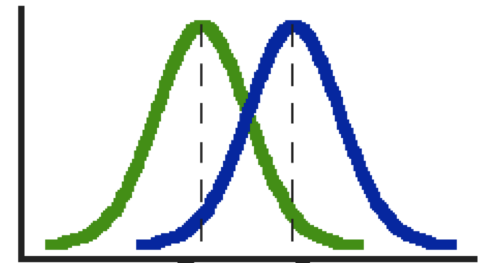
\includegraphics[width=0.7\linewidth]{t-student}

\textbf{Hipótesis} H0 : \(\mu_1\) = \(\mu_2\) H1 : \(\mu_1\) r \(\neq\)
\(\mu_2\)

\textbf{Supuestos:} 1) Las variables X es continua. 2) Distribución
normal.
\end{frame}

\begin{frame}{R Documentation Student's t.test \{stats\}}
\protect\hypertarget{r-documentation-students-t.test-stats}{}
t.test(x, y = NULL,\\
alternative = c(``two.sided'',``less'',``greater''),\\
paired = FALSE,\\
var.equal = FALSE,\\
conf.level = 0.95, \ldots)

\textbf{Two Sample t-test} data: Peso by Sexo\\
t = -11.315, df = 18, p-value = 1.292e-09\\
alternative hypothesis: true difference in means is not equal to 0\\
95 percent confidence interval:\\
-41.18421 -28.28530\\
sample estimates:\\
mean in group Female 141.9380 mean in group Male 176.6727
\end{frame}

\begin{frame}{PRÁCTICA ANÁLISIS DE DATOS}
\protect\hypertarget{pruxe1ctica-anuxe1lisis-de-datos}{}
\begin{itemize}
\item
  Guía de trabajo práctico disponible en drive y Rstudio.cloud.\\
  \textbf{Clase\_10}
\item
  El trabajo práctico se realiza en Rstudio.cloud.\\
  \textbf{10 Inferencia estadística}
\end{itemize}
\end{frame}

\begin{frame}{RESUMEN DE LA CLASE}
\protect\hypertarget{resumen-de-la-clase}{}
\begin{itemize}
\item
  \textbf{Elaborar hipótesis}
\item
  \textbf{Realizar pruebas de hipótesis}

  \begin{itemize}
  \tightlist
  \item
    Test de correlación.\\
  \item
    Test de comparación de medias para 2 muestras independientes.
  \item
    Test para muestras pareadas.
  \end{itemize}
\item
  \textbf{Realizar gráficas avanzadas con ggplot2}
\end{itemize}
\end{frame}

\end{document}
